\section{Einleitung}

In dieser Ausarbeitung soll eine Methode beschrieben werden, mit deren Hilfe man durch endlich viele Zufallszahlen 
eine ungefähr gleichmäßige Verteilung von Punkten im Raum erzeugen kann. Damit kann man sehr gut Daten simulieren, 
welche eine bestimmte Verteilung besitzen und, wie in der Natur üblich, keine harten Kanten besitzen oder komplett 
zufällig verteilt sind, sondern langsam abfallend strukturiert sind. Zu diesen Dichteverteilungen gehört zum Beispiel 
auch die Gaußschen Normalverteilung. 

Falls nicht anders beschrieben, werden in dieser Ausarbeitung für die randomisierten Eingaben sogenannte "Golden Ratio Sequences"
verwendet. Diese wurden von Schretter \cite{schretter-golden_ratio_sequences-2012} vorgestellt und verteilen zufällig 
uniform verteilte Punkte im $[0, 1]$-Quadrat, wie in \ref{fig:grs500} zu sehen ist. Durch die Inversionsmethode \cite{devroye-non_uniform_random_variate-1986} 
können diese Punkte dann auf alle möglichen Größen und Verteilungen gekrümmt werden. Deshalb werden diese gleichmäßig 
verteilten Punkte auf die von Chen und Asau \cite{chen_asau-generating_random_variates-1974} und Devroye 
\cite{devroye-non_uniform_random_variate-1986} beschriebene, verbesserte \hyperref[funktion]{Inversionsmethode} mit Hashing 
angewandt, wodurch das gewünschte Ergebnis erzielt wird. Diese Verfahrenskette wird unter \hyperref[impl]{Implementation} 
näher erläutert und durchgeführt. 


\subsection{Problemstellung}
Mithilfe dieser Arbeit über die Hash-basierte Inversionsmethode, soll gezeigt werden, wie diese funktioniert und ob  
sie bei der Generierung von multivariaten Verteilungen in höheren Dimensionen mithilfe von uniformen Dichten immer noch 
korrekt arbeitet und einsetzbar ist. Außerdem soll verglichen werden, ob sich der Einsatz der hier beschriebenen 
Methode als Ersatz von bereits existierenden anderen Methoden lohnt. 

\begin{figure}
    \centering
    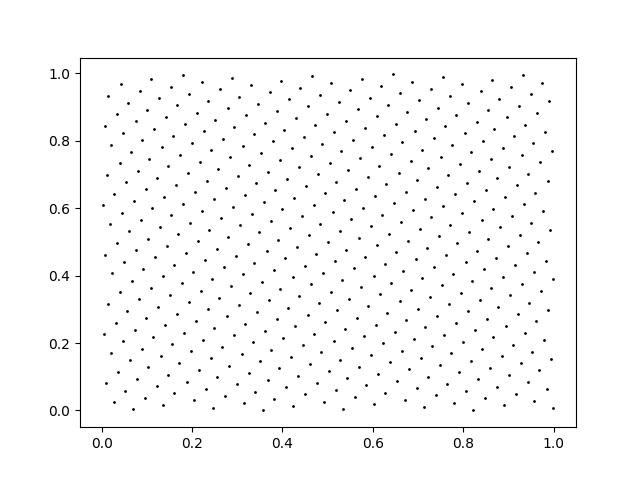
\includegraphics[width=.45\textwidth]{pdf_plots/grs_u500c}
    \caption{500 gleichmäßige, zufällige Punkte einer Goldenen-Schnitt-Sequenz \cite{schretter-golden_ratio_sequences-2012}.}
    \label{fig:grs500}
\end{figure}

\subsection{Stand der Technik}
Um das Inverse einer Funktion anzunähern, kann nicht nur die hash-basierte Inversionsmethode verwendet werden, sondern 
beispielsweise auch ein Feld der Partialsummen der einzelnen Wahrscheinlichkeiten, einen Punkt an einer bestimmten Stelle anzutreffen. 
Auf diesem Feld können dann wiederum unterschiedliche Methoden zum Finden der passenden Werte verwendet werden. Dazu gehören 
lineare Suche von vorne nach hinten, binäre Suche oder auch ein Huffman-Baum.

Zur Generierung uniformer Zufallszahlen gibt es anstelle der Sequenzen des goldenen Schnittes auch Methoden wie
die von Halton \cite{wong_luk_heng-halton_points_sampling-1997}, sogenannten Blue Noise \cite{yan-blue_noise_sampling-2015} 
oder Rang-1-Gitter \cite{prasad-rank1lattice-1973}. Doch da Schretter in seinem Paper zeigt, dass die von diesen Methoden generierten Zahlen 
nicht so gleichmäßig verteilt werden, wie von seiner neuen Methode \cite{schretter-golden_ratio_sequences-2012}, 
wird hier diese verwendet. 